\documentclass[final]{lktseminar}

% ------------------------------------------------
%  Preamble / Praeambel
% ---------------------
%Text-Encoding
%\usepackage[latin1]{inputenc} %latin1
\usepackage[utf8]{inputenc} %UTF-8
\usepackage[ngerman]{babel}

%Stil der Zitate und der Bibliographie
\usepackage[style=numeric-comp]{biblatex}
\nocite{*}
%Bibliographie laden:
\addbibresource{literature.bib}

%
\graphicspath{{./images/}}

% Satz aufhuebschen
\clubpenalty=10000  % Keine Schusterjungen, Hurens"ohne
\widowpenalty=10000

%Silbentrennung:
% Liste von unbekannten und zusammengesetzten Woertern.
%Bei Woerter mit Bindestrich ist das ...-... durch ...''=... zu ersetzen -> weitere Informationen:
% http://de.wikibooks.org/wiki/LaTeXWoerterbuch:_Silbentrennung
\hyphenation {%
}
% ------------------------------------------------



% ------------------------------------------------
%  ... / Dokument

\begin{document}
% ------------------------------------------------
% .../Informationen
% -----------------
\myname{Biesinger Christoph}
\mytitle{IP-Pakete "uber IEEE 802.15.4-Netzwerke}
\myshorttitle{IP-Pakete "uber IEEE 802.15.4-Netzwerke}
\mymatnr{1350722}
\mystudycourse{Masterstudiengang Informatik}
\myreviewer{M.Sc. Dario Fanucchi}
% ------------------------------------------------

% Setting of language
\selectlanguage{ngerman}
%\selectlanguage{english}

\makeAuthor
\makeTitle
\makeInfos
\maketitle

% ------------------------------------------------
% Abstract / Kurzfassung
% ----------------------
\begin{abstract}
\section*{Kurzfassung}

IP-Pakete "uber IEEE 802.15.4-Netzwerke beschreibt eine Netzwerktechnologie f"ur das Internet Protocol Version 6 IPv6,
IPv6 over Low-Power Wireless Personal Area Networks 6LoWPAN. 6LoWPAN bildet eine Adapationsschicht zwischem dem Data Link und
Network Layer, welche als notwendige Grundlage dient um die Low-Rate Wireless Personal Area Networks LR-WPANs des Internet
der Dinge IoT mit den bereits bestehenden Netzwerken "uber IPv6 zu verbinden. Daher werden verschiedene Mechanismen, wie
 Headerkompression und mehrere Verfahren f"ur Routing ausgebildet, womit ein Kommunikationsprotokoll und Standard um
 den kommenden Entwicklungen des Internet der Dinge gen"ugezuleisten.

\end{abstract}
% ------------------------------------------------

\newpage

% ------------------------------------------------
% ... / Inhaltverzeichnis
% -----------------------
\tableofcontents
% ------------------------------------------------

\newpage

% Abbildungsliste
\listoffigures
\newpage

% ------------------------------------------------
% ... / Einleitung
% ---------------

% --------------------------------------
\section{Einleitung}
\label{sec:Einleitung}

\subsection{Motivation}
\label{sec: Motivation}
Aktuell entwickelt sich ein neuer Trend im Bereich der Informations- und Kommunikationstechnologien, unter dem Begriff des
``Internet of Things" kurz IoT, indem sukzessiv Alltagsgegenst"ande mithilfe von Mikrocontrollern zu
``intelligente Gegenst"ande" transformiert werden, womit die Grenze zwischen realer und virtueller Welt zunehmend verwischen soll.
Das IoT ist in seiner Idee ein allumfassendes Kommunikationssystem, bei dem die Netzwerkknoten nicht mehr durch die
Verwendung von Benutzern charakterisiert werden, sondern durch autonom agierende ``Dinge".
Der technische Hintergrund ist, dass eine Vielzahl von eingebetteten Systemen, mit begrentzten Ressourcen und Kapazit"aten
 an Rechnerleistung und Stromverbrauch, Informationen sammeln und erzeugen. Diese sollen dar"uberhinaus
miteinander verbunden sein und ein globales Netzwerk erzeugen, sprich das ``Internet der Dinge".
Diese Eingebetten Systeme sollen dabei in sehr gro"ser Anzahl "uber alle Bereiche des Lebens und an alle Orte verteilt werden
und die Anzahl der bestehenden Benutzersysteme wie Computer, Smartphones oder Tablets um mehrere Gr"o"senordnungen
"ubersteigen.

Dieser Trend soll dabei nicht nur in das allt"agliche Privatleben eindringen, sondern auch im Rahmen der Initiative
``Industrie 4.0" das Wirtschaftsleben mit "intelligenten Fabriken" revolutionieren, indem diese dynamisch auf Ver"anderungen
regieren. Deshalb wird ist eine Netzwerktechnologie n"otig, die sowohl die Anforderungen der Hardware mit der
bereits vorhandenen Netzwerkstruktur verbindet, weshalb die Internet Engineering Task Force IETF den 6LoWPAN Standard
geschaffen hat.

% --------------------------------------

\subsection{IEEE 802.15.4-Netwerke - Low-Rate Wireless Personal Area Networks}
\label{sec: 802.15.4-Netwerke - Low-Rate Wireless Personal Area Networks}

Das technische Grundger"ust des IoT bilden die verwendeten Rechnernetzwerke, zur Erstellung dieser Netzwerke
werden verschiedene Technologien verwendet. Daf"ur wurden viele verschiedene Technologien entwickelt, wie beispielsweise
 Radio-Frequency IDentification RFID, Wirless Sensor Networks WSN oder Bluetooth, wobei wir uns in dieser
 Arbeit auf den IEEE 802.15.4 Standard beschr"anken, welches Low-Rate Wireless Personal Area Networks LR-WPANs beschreibt.
 LR-WPANs m"ussen dabei bestimmte Anfoderungen erf"ullen, da sie abh"angig von den Beschr"ankungen der verwendeten
 Cyber-Physikalischen Systeme sind, welche als Hardwaregrundlage fungieren. Diese LR-WPAN-Eigenschaften sind dabei, \dots
\begin{itemize}
    \item eine einfache Architektur f"ur drahtlose Kommunikationsnetzwerke
    \item begrenzte Kapazit"at an Stromverbrauch (batteriebetrieben), Datendurchsatz (bis 250 kb/s) und Reichweite (weniger als 100 Meter)
    \item kleine Paketgr"osse (127 Bytes) auf dem IEEE 802.15.4 Frame
    \item Unterhalt einer hohe Anzahl an unzuverl"assigen Ger"aten durch Ver"anderung der physikalischen Gegebenheiten
    \item Unterst"utzung verschiedene Topologiearten: Mesh, Stern und Peer-to-Peer
\end{itemize}

Der IEEE 802.15.4 Standard spizifiziert dabei den Physical Layer (PHY) und den Media Access Control Layer (MAC) des
OSI-Referenzmodells f"ur LR-WPANs.
Die PHY-Schicht stellt dabei die "Ubertragung von PHY protocol data units PPDUs "uber die verwendeten drahtlosen physikalischen Medium sicher,
wobei zwei Arten von Ger"atetypen unterschieden werden k"onnen. Den Reduced Function Devices RFD, den typischen batteriebetrieben Ger"aten
innerhalb des IoT, und den Full Function Devices FFD, leistungsf"ahiger Hardware mit Stromanschluss. Letztere k"onnen Nachrichten innerhalb des
Netzwerkes weiterleiten und werden an zu PAN Koordinatoren (Personal Area Network) sollten sie die Organisation des ganzen Netzwerkes
"ubernehmen. Aufgrund dieser Eigenschaften und Aufgaben wird das Netzwerk oft zu einem vermaschten Netzwerk (Mesh Network) ausgebaut.
Die MAC-Schicht ist f"ur die Daten"ubertragung und den Empfang mitsamt Verwaltung verantwortlich, wie die Validierung der Frames und dem
Beacon Management.

\begin{figure}[h]
    \centering
    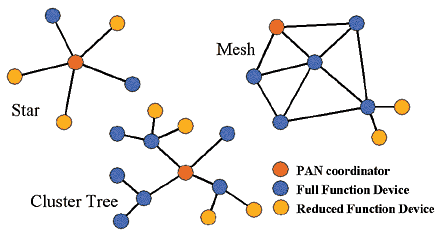
\includegraphics[scale=0.7]{mesh_network.png}
    \caption{Mesh Network \cite{mesh_network_picture}}
    \label{fig:Mesh Network}
\end{figure}

Dadurch bildet der Standard die Basis f"ur die Dienste der Netzwerkschicht wie IPv6 over Low-Power Wireless Personal Area Networks 6LoWPAN.


\newpage
% --------------------------------------
% Kapitel 2 - 6LoWPAN
% --------------------------------------

\section{6LoWPAN: IPv6 over Low power Wireless Personal Area Network}
\label{sec: 6LoWPAN: IPv6 over Low power Wireless Personal Area Network}

6LoWPAN steht f"ur IPv6 over Low-Power Wireless Personal Area Networks und beschreibt eine Netwerktechnologie
und Adaptionsschicht f"ur IPv6 Pakete "uber 802.15.4-Netwerke. Im folgenden Kapitel wird nun
die urspr"ungliche Zielsetzung der verantwortlichen Workgroup \ref{sec: Urspr"ungliche Zielsetzungen}
 und die grundlegenden Charakteristiken \ref{sec: Charakterisierung von 6LoWPAN} vorgestellt.
Anschlie"send wird 6LoWPAN im Detail anhand den 6LoWPAN Header \ref{sec: 6LoWPAN Header} mitsamt dem
``Stacked Header Prinzip'' betrachtet. Das letzte Unterkapitel \ref{sec: IPv6 Header Compression}
behandelt schlie"slich den Kompressionsmechanismus f"ur IPv6 Header.

% --------------------------------------


\subsection{Urspr"ungliche Zielsetzungen}
\label{sec: Urspr"ungliche Zielsetzungen}

LoWPANs bestehen wie im vorherigen Kapitel \ref{sec: 802.15.4-Netwerke - Low-Rate Wireless Personal Area Networks}
beschrieben, aus einfachen Netzwerkknoten mit begrentzten Kapazit"aeten. Gerade da diese Netzwerke mitsamt
 ihren Ger"aten f"ur k"unftige Technologien wie IoT  und ``Industrie 4.0''
 gedacht sind, bot es sich an, diese Netzwerke mittels Internet Protocol Version 6 IPv6 zu verbinden.
 Dar"uberhinaus folgte man dem Ansatz, m"oglichst das zu Benutzen, was bereits vorhanden war.

 W"ahrend der Entwicklung f"ur eine angepasste Version von IPv6 wurden daher
 einige Vorgaben\cite{rfc4919} definert, welche anhand den IEEE 802.15.4-Netzwerken
 ausgerichtet sind. Diese w"aren, die Reduzierung des Paket-Overheads von IPv6,
 ein geringerer Verbrauch von Bandbreite und Strom, sowie m"lgichst geringe Anforderungen
 and die Rechnerkapazit"at.

Anhand diesen Vorgaben, wurden nun folgende Ziele f"ur die Umsetzung von 6LoWPAN definiert, \dots
\begin{itemize}
    \item Erstellung eines Fragmentation und Assembly Layers, zur Kombination von
    LR-WPANs und IPv6.
    \item Ein Mechanismus zur Kompression des Headers, sowie die Nutzung des Network
    Management, von IPv6.
    \item Erschaffung eines Mesh Routing Protokolls, anhand von LR-WPANs.
    (siehe Kapitel \ref{sec: RPL Ripple} bzgl. Routing Protocol for Low power and Lossy Networks)
\end{itemize}


% --------------------------------------


\subsection{Charakterisierung von 6LoWPAN}
\label{sec: Charakterisierung von 6LoWPAN}

Anhand der Vorgaben und Zielsetzungen, k"onnen nun die eindeutigen Charakteristiken von 6LoWPAN abgeleitet werden.
\begin{description}
    \item[IPv6-Stack als Grundlage] Der Hauptgrund an der Verwendung von IP-basierter
    Technologie, beruft sich sowohl an der Bekanntheit, dass die weltweite Entwicklergemeinde
    Erfahrungen mit dem Protokoll aufweisen kann, IPv6 eine bereits bew"ahrte Technologie verk"orpert
    und das auf eine bereits bestehende Infrastruktur aufgebaut werden kann. Dies wird auch
    erweitert durch die Verwendung von TCP/IP.

    \item[Eigenschaften von IPv6] Zus"atzlich bietet IPv6 eine kosteneffektive Nutzung, da es geringe
    Kosten bei der Implementierung, der Protokoll-Komplexit"at, der ben"otigten Konfigurations Infrastruktur
    und dem Header/Protokoll-Overhead aufweist.

    \item[Stacked Header Prinzip] Dieses Prinzip beschreibt die Erstellung von mehreren Typen an Headern,
    welche gestapelt (stacked) werden k"onnen und somit verschiedene Anforderungen erf"ullen k"onnen. Daher
    besitzt 6LoWPAN vier verschiedene Header-Typen, welche im Kapitel \ref{sec: 6LoWPAN Header} im Zusammenspiel und
    einzeln erkl"art werden. Die Notwendigkeit zur Verwendung dieses ``Stacked Header Prinzip" wird im folgenden Unterkapitel
    \ref{sec: Maximum Transmission Unit MTU} erl"autert.

    \item[Routing M"oglichkeiten] 6LoWPAN arrangiert zwei Varianten zum Routing von Paketen.
    Die erste Variante ist das traditionelle Routing per Network Layer mittels Routing Protokoll (Route-Over)
    oder alternativ ein Data Link Layer Routing mittels MAC-Adressen(Mesh-Under). Eine genaue Erkl"arung der
    Varianten und deren Unterschied werden im Kapitel \ref{sec: 6LoWPAN Routing} genauer erl"autert.

    \item[Kompressions Mechanismus] Kompression der IPv6-Header mittels eines Mechanismus, basierend
    auf dem Stacked Header Prinzip zur Reduzierung der Paket-Gr"o"se. Eine genaue Beschreibung erfolgt
    im Kapitel \ref{sec: IPv6 Header Compression}.

\end{description}
% --------------------------------------

\subsubsection{Maximum Transmission Unit MTU}
\label{sec: Maximum Transmission Unit MTU}

Durch die Verbindung von Internet Protocol Version 6 und IEEE 802.15.4-Netzwerken innerhalb
von 6LoWPAN, m"ussen verschiedene Anforderungen an die Maximum Transmission Unit MTU\cite{rfc4944}
gleichzeitig erf"ullt werden. Dabei erm"oglicht IPv6 Pakete mit einer MTU von bis zu 1280 Bytes,
wobei LR-WPAN Frames aufgrund ihres Headers, sowie der AES-CCM-128 Verschl"usselung nur
maximal 81 bytes f"ur die dar"uberliegende Schicht bereitstellen.
Deshalb wird ein Adapations Layer ben"otigt, welcher Pakete fragmentiert und wieder zusammensetzt.

Zus"atzlich folgt, dass der IPv6 Header weitere 40 Bytes und ein Transportprotokoll wie UDP
weitere 8 Bytes beansprucht, wodurch nur noch weitere 33 Bytes f"ur die eigentliche Anwendung verf"ugbar w"are.

Deshalb m"ussen folgende Betrachtungen ber"ucksichtigt werden:

\begin{itemize}
    \item Ein Adaption Layer muss die Anforderungen bez"uglich der MTU von IPv6 (1280 Bytes) und LR-WPAN (81 Bytes) beachten.
    \item Ein Mechanismus zur Kompression der Header ist zwingend notwendig.
\end{itemize}

Die L"osung dieser Probleme wird durch die 6LoWPAN Header aufgrund des Stacked Header Prinzips und dem
 Kompressionsmechanismus durch das LOWPAN\_IPHC Encodingformat umgesetzt.
% --------------------------------------
\newpage


\subsection{6LoWPAN Header}
\label{sec: 6LoWPAN Header}

Die 6LoWPAN Header, Dispatch Header \ref{sec: Dispatch Header}, Mesh Header \ref{sec: Mesh Header},
Fragmentation and Assembly Header \ref{sec: Fragmentation and Assembly Header} und das
LOWPAN\_IPHC Encodingformat \ref{sec: IPv6 Header Compression}, bilden zusammen die Adaptionsschicht zwischen dem Data Link Layer,
symbolisiert durch das IEEE 802.15.4-Frame, und dem Network layer, repr"asentiert durch IPv6 Pakete,
siehe Abbildung \ref{fig:Vergleich Stack-Modelle}. Diese Adapationsschicht wird wird mit Hilfe
des ``Stacked Header Prinzip'' umgesetzt, bei dem die verschiedenen 6LoWPAN Header aneinandergereiht
werden um die jeweiligen Header-Informationen darzustellen. Die Header werden dabei durch den
2 Bit langen vordefinierten Type Identifier unterschieden. Durch dieses Prinzip werden nur die Informationen gesendet,
welche ben"otigt werden und unn"otige Headerteile werden ausgespart. Direkte Anwendung des
``Stacked Header Prinzip" werden im Kapitel \ref{sec: Kommunikationsszenarien} anhand von
Beispielen weiter verdeutlicht.

\begin{figure}[h]
    \centering
    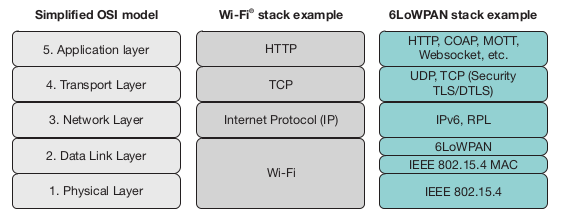
\includegraphics{6lowpan_osi_stack.png}
    \caption{Vergleich OSI-Referenzmodell, Wi-Fi Stack und 6LoWPAN-Stack \cite{6lowpan_demystified}}
    \label{fig:Vergleich Stack-Modelle}
\end{figure}

% --------------------------------------

\subsubsection{Dispatch Header}
\label{sec: Dispatch Header}

Der Dispatch Header hat eine Aufgabe, die Beschreibung der auf ihn folgenden Headertypen anhand der verwendeten
Kompression. Der 1 Byte gro"se Header ist dabei in zwei Felder aufgeteilt, zuerst den 2 Bit langen
 Type Identifier (01) gefolgt von dem 6 Bit langen Dispatch Value.
 Dieser Wert beschreibt dabei einen vordefinierten anderen Header Typ, wie in der darauffolgenden Abbildung
\ref{fig:Dispatch Header} zu sehen ist.

\begin{figure}[h]
    \centering
    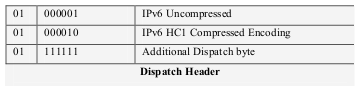
\includegraphics{dispatch_header.png}
    \caption{Dispatch Header \cite{6lowpan_architecture}}
    \label{fig:Dispatch Header}
\end{figure}

% --------------------------------------

\subsubsection{Mesh Header}
\label{sec: Mesh Header}

Der Mesh Header codiert das Hop Limit des Paketes sowie die Quell- und Zieladresse des Frames auf dem Data Link Layer.
Dadurch beinhaltet der Mesh Header alle n"otigen Informationen f"ur ein einfaches aber effektives Routing mittels
MAC-Adressen, wobei ein einfaches Mesh Netzwerk erstellt wird, deshalb nennt sich dieses Verfahren ``Mesh-Under''.
Zus"atzlich bietet der Mesh Header durch IEEE 802.15.4 die M"oglichkeit, die kurzen 16 Bit Adressen zu verwenden, anstatt
den normalen 64 Bit Adressen.
Daher erfolgt die Aufteilung des Headers in:
\begin{itemize}
    \item den Type Identifier (01), 2 Bit
    \item die Angabe der Adressenl"ange, seperat f"ur Quelladresse (O) und Zieladresse (F). Jeweils 1 Bit.
    \item das Hop Limit, 4 Bit
    \item sowie der Quell- und Zieladresse (32 - 128 Bit)
\end{itemize}

\begin{figure}[h]
    \centering
    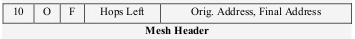
\includegraphics{mesh_header.png}
    \caption{Mesh Header \cite{6lowpan_architecture}}
    \label{fig:Mesh Header}
\end{figure}
% --------------------------------------

\subsubsection{Fragmentation and Assembly Header}
\label{sec: Fragmentation and Assembly Header}

Die Notwendigkeit f"ur den Fragmentation and Assembly Header wurde bereits im Kapitel \ref{sec: Maximum Transmission Unit MTU} ausgiebig erl"autert,
wodurch sich f"ur den Header mehrere Charakteristiken ergeben, welche zu folgendem Aufbau des Headers f"uhren, \dots
\begin{itemize}
    \item dem Type Identifier (11), 2 Bit
    \item Angabe ob sich um das erste Fragment (000) oder ein darauffolgendes Fragment (100) handelt, 3 Bit
    \item Die Datagram Size gibt die L"ange des gesamten IP Paketes vor der Fragmentation auf dem Data Link Layer an.
    Dieses Feld ist f"ur folgende Pakete optional und kann daher weggelassen werden. 11 Bit.
    \item Der Datagram Tag beschreibt eine eindeutige Nummer, welche f"ur alle Fragmente des IPv6 Datagrams verwendet wird.
    Dadurch werden die einzelnen Frames auf der Empf"angerseite zugeordnet. 16 Bit.
    \item Das letzte Feld wird nur im zweiten und den darauffolgenden Fragmenten verwendet und entspricht einer Sequenznummer
    um die richtige Reihenfolge der Fragmente zu gew"ahrleisten. 8 Bits.
\end{itemize}

\begin{figure}[h]
    \centering
    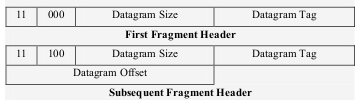
\includegraphics{fragment_header.png}
    \caption{Fragmentation Header \cite{6lowpan_architecture}}
    \label{fig:Fragmentation Header}
\end{figure}

% --------------------------------------

\subsubsection{Kommunikationsszenarien}
\label{sec: Kommunikationsszenarien}

Im folgenden werden drei Kommunikationsszenarien vorgestellt, welche das Stacked-Header-Prinzip erl"autern.
\begin{figure}[h]
    \centering
    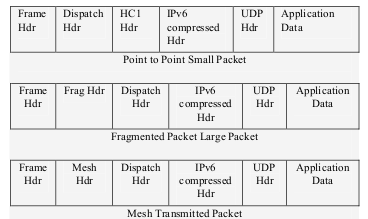
\includegraphics{kommunikationsszenario.png}
    \caption{Verschiedene Kommunikationsszenarien \cite{6lowpan_demystified}}
    \label{fig:Kommunikationsszenarien}
\end{figure}

\begin{itemize}
    \item Das erste Beispiel beschreibt eine einfache Kommunikation mit Point-to-Point Small Packets. Dabei wird nur
    der Dispatch und LOWPAN\_IPHC Header verwendet, sowie der komprimierte IPv6 Header welcher lediglich 2 Bytes l"ange. Die beiden
    6LoWPAN Header beanspruchen zusammen ebenfalls nur 2 Bytes.
    \item Das n"achste Szenario beschreibt das erste fragmentierte Teilpaket eines gro"sen Paketes. Dabei wird vor dem Dispatch Header der
    Fragmentation Header auf dem Data Link Layer verwendet.
    \item Das letzte Beispiel erl"autert ein Paket welches ``uber ein Mesh Netzwerk transportiert wird.

\end{itemize}
% --------------------------------------
\newpage
\subsection{IPv6 Header Compression}
\label{sec: IPv6 Header Compression}

Die Grundlage f"ur die Kompression des IPv6 Headers ist das Codierungsformat LOWPAN\_IPHC \cite{rfc6282}.
LOWPAN\_IPHC gew"ahrleistet dabei eine effektive Komprimierung von lokalen, globalen und Multicast IPv6 Adressen,
basierend auf geteilten Informationen, Felder des IPv6 Headers, innerhalb des Kontext von 6LoWPAN.
Damit werden Informationen, welche von IEEE 802.15.4-Netzwerken auf dem Data Link Layer und IPv6 auf dem Network Layer,
redundant existieren innerhalb von 6LoWPAN kombiniert. Dadurch kann der, im Kontext sehr gro"se, IPv6 Header
deutlich komprimiert werden.

Im folgenden k"onnen nun die Informationen des IPv6 Headers von urspr"unglich 40 Byte schrittweise komprimiert werden,
indem diese Informationen durch Annahmen mit festen Werten gef"ullt werden (Version, Traffic Class und Flow Label)
oder durch Informationen aus dem IEEE 802.15.4 Frame ersetzt werden(Payload Lenght, Next Hop).

\begin{description}
    \item[LOWPAN\_IPHC Codierungsformat] Das LOWPAN\_IPHC Codierungsformat beschreibt wie der IPv6 Header komprimiert wird.
    Bei dem Standard Encoding, entspricht das Codierungsformat einem Header von 2 Byte breite.
    Sollte f"ur IPv6 das Additional Context Feld aktiv sein, nimmt der LOWPAN\_IPHC Header 3 Byte ein.
    Im Grunde entspricht der LOWPAN\_IPHC Header dabei einem reinen Flag-Feld und gibt mit einzelnen Bits oder Bitfolgen an,
    ob Felder des IPv6 Header komprimiert werden bzw. wie diese Komprimierung stattfindet.

    Die wichtigsten Felder sind dabei, \dots
    \begin{itemize}
        \item die Bitfolge 011, welche den LOWPAN\_IPHC Header einl"autet.
        \item das HLIM-Feld (2 Bit), welches die Gr"o"se des Hop Limit angibt,
        \item das SAC bzw. DAC Feld (1 Bit), gibt die Kompression f"ur Source bzw. Destination Adresse an.
        \item sowie das SAM bzw. DAM Feld (2 Bit), erl"autert die L"ange der Adressen an.
        (16-Bit Adressen weren durch die Kombination ``10" angegeben)
    \end{itemize}
\end{description}

Der Hauptpunkt der Kompression liegt dabei in den IPv6 Adressen\cite{rfc4291}, welche eine L"ange von 128 Bit aufweisen. Diese
Adresse ist dabei grundlegend in zwei Bereiche aufgeteilt. Die erste H"alfte von 64 Bit, wird als Pr"afix bezeichnet und
steht f"ur das angeschlossene Subnetz. Die zweite H"alfte von 64 Bit, ist der Interface-Identifier IID und ist
gleichzusetzen mit der MAC-Adresse.

Aufgrund dieser Tatsache muss bei der Kompression der IPv6 Adressen besonders betrachet werden, wobei sich Unterschiede
bei der Reichweite (Anzahl der Hops) des IP-Pakets aufzeigen.

\begin{description}
    \item[Kommunikation "uber einen (1) Hop] bezeichnet den einfachsten Fall und entspricht dem ``Best Case" f"ur
    LOWPAN\_IPHC Kompression. Da der Suffix der IPv6-Adresse der MAC-Adresse auf dem Data Link Layer entspricht, wird
    diese Information vom IEEE 802.15.4 Frame ``ubernommen. Der Pr"afix kann bei einer Link Local-Adresse sogar komplett
    weggelassen werden, womit von dem IPv6 Header nur 3 Bytes ``ubrigbleiben, 1 Byte Dispatch Header, 1 Byte LOWPAN\_IPHC Encoding Feld
    und 1 Byte f"ur das Hop Limit Feld, welches als einziges ohne ``Anderungen ``bernommen wird. Damit wurden 37 Byte des
    urspr"unglichen IPv6 Header gespart, dies entspricht eine Kompression von 92,5 Prozent.

    \item[Kommunikation "uber mehrere (\textgreater 1) Hops] unterscheidet sich zur Kommunikation ``ber einen Hop nur anhand der MAC-Adressen.
    Diese sind innerhalb mehreren Hops nicht identisch weshalb der Suffix angegeben werden muss. Dabei k"onnen nun die langen 64-Bit Adressen oder die
    kurzen 16-Bit Adressen gew"ahlt werden. Der Pr"afix kann innerhalb eines Subnetzes (Verbindung mit Link Local-Adresse) weggelassen werden.
    Damit ergibt sich f"ur den IPv6 Header eine L"ange von 7 Byte, zusammengesetzt aus Dispatch Header (1 Byte), LOWPAN\_IPHC Feld (1 Byte),
    HOP Limit Feld (1 Byte), sowie der Quell- und Zieladresse (jeweils 2 Byte). Dies entspricht eine Reduktion von 33 Byte durch
    Kompression, wodurch 82,5 Prozent gespart wurden.
\end{description}

Im urspr"unglichen Design der Kompression \cite{rfc4944} wurden die Kompressionsheader LOWPAN\_HC1 und LOWPAN\_HC2 vorgestellt.
Diese wurden sp"ater durch LOWPAN\_IPHC \cite{rfc6282} ersetzt, da sie f"ur  die praktische Umsetzung unzureichend waren.
\begin{description}
    \item[HC1 Encodingformat] HC1 Coding beschreibt die Kompression des IPv6 Headers anhand eines 8 Bit langen
    Feld-Header. Dieser LOWPAN\_HC1 Header gibt an, wie mit den IPv6 Header Felder umgegangen wird und
    welches Protokoll IPv6 nachfolgt (UDP, TCP, ICMP). Im letzteren Fall kann zus"atzlich das LOWPAN\_HC2 Encodingformat
    angewendet werden, welches einen LOWPAN\_HC2 Header an den LOWPAN\_HC1 Header anschlie"st, und die Kompression
    f"ur das anschlie"sende Transportprotokoll angibt.

    \item[Grundlage f"ur Austausch] N"otig wurde ein anderes Codierungsformat, da HC1 Encoding Probleme mit der Kompression
    der Adressen aufzuweisen hat. Im Idealfall f"ur HC1 Encoding, der Verwendung von Link Local-Adressen (Mesh-Under Routing),
    k"onnen die die IPv6 Adressen vollst"andig gespart werden. Dieser Wegfall beeinflusst zwar nicht das Routing auf der
    Netzwerkschicht, da IPv6 Neighbor Discovery und Routing Protokolle ebenfalls mit Link Local-Adressen funktionieren, aber
    Kommunikationsverbindung auf h"oheren Schichten sind von IPv6 Adressen abh"angig. Bei Route-Over Routing und der deshalb
    n"otigen Nutzung von IPv6 Adressen, werden diese nur auf 64 Bit komprimiert, da der Interface Identifier IID angegeben werden
    muss und dieser nicht f"ur die kurzen 16-Bit Adressen von IEEE 802.15.4 geeignet ist. Bei Multicast Verbindung muss sogar
    die vollst"andige IPv6 Adresse angegeben werden, wodurch 128 Bit Traffic entsteht.
\end{description}

% TODO Next Header Compression

% --------------------------------------

%\subsection{Softwareimplementierung und Hardware}
%\label{sec: Softwareimplementierung und Hardware}

%In-Depth Breakdown of a 6LoWPAn Stack for Sensor Networks - Sergio Lembo, Kuusisto, Manner
%\url{http://airccse.org/journal/cnc/1110ijcnc14.pdf}

%contiki
%small to tiny cpus
%unterstuetzt ipv6, 802.15.4, 6lowpan
%kein real-time, statt dessen protothreads

%tinyos
%tinyos alliance
%staerkere hardware als contiki (atmega128)

% --------------------------------------
% Kapitel 3 - Routing
% --------------------------------------

\section{6LoWPAN Routing}
\label{sec: 6LoWPAN Routing}

Dieses Kapitel behandelt das Routing f"ur 6LoWPAN. Dabei wird zuerst auf die zwei verschiedenen
Kategorien des 6LoWPANs Routing, Route Over vs. Mesh Under \ref{sec: Route Over vs. Mesh Under} behandelt.
Im n"achsten Schritt, wird das Routing Protokoll der Netzwerkschicht RPL Routing Protocol for Low power and Lossy Networks
\ref{sec: RPL Ripple} beispielhaft betrachtet.
% --------------------------------------

\subsection{Route Over vs. Mesh Under}
\label{sec: Route Over vs. Mesh Under}


Routing ist ein wichtiges Thema, da Knotenpunkte begrentzte F"ahigkeiten besitzen, siehe LR-WPAN
\ref{sec: 802.15.4-Netwerke - Low-Rate Wireless Personal Area Networks},
weshalb verschiedene Routing-Protokolle entworfen wurde. Diese k"onnen dabei in zwei
Kategorien eingeteilt werden.
\begin{description}
    \item[Mesh Under] beschreibt das Routing auf dem Adaption Layer von 6LoWPAN, wodurch
    das Routing auf dem Data Link Layer, mit Hilfe der kurzen 16-Bit oder der Standard-64-Bit langen MAC Adressen stattfindet.
    Daf"ur wird der Mesh Header\ref{sec: Mesh Header} den restlichen 6LoWPAN Headern,
    wie dem Fragmentation and Assembly Header sowie dem Dispatch Header vorangstellt.
    Wobei mehrere Link Layer Hops einen einzelnen IP Hop ersetzen, damit entspricht die Reichweite einer IPv6 Verbindung
    alle Knoten im gleichen Multihop Mesh. Bei einem fragmentierten Paket werden die einzelnen Fragmente
    "uber den Mesh, evtl. auf unterschiedlichen Routen, geschickt und am Ziel gesammelt und
    bei Eintreffen aller Fragmente wieder zusammengesetzt.

    \item[Route Over] ist das Standard IP-Routing auf dem Network Layer, dabei wird jeder Knoten
    auf dem Data Link Layer als als IP Router betrachtet, womit ein Hop auf dem Data Link Layer einem
    Hop auf dem Network Layer entspricht, daher spiegelt diese einzige Verbindung die Reichweite der IPv6 Verbindung dar.
    Damit k"onnen nun die Dienste von IPv6 bzgl. Routing, wie Routing Tabellen und Hop-by-Hop Optionen
    angewendet werden. Der Adaptions Layer von 6LoWPAN ``ubernimmt in diesem Fall das Mapping zwischen
    den beiden Layern und sorgt haupts"achlich f"ur das Fragmentieren und Zusammensetzen der Pakete.
    Zusammengefasst besteht das Route Over Netzwerk aus mehreren sich "uberlappenden Link Local Bereichen,
    wobei jeder Knoten seinen eigenen Link Local Bereich, mit in direkten Verbindung stehenden Nachbarn, besitzt.
    F"ur diesen Fall wird im folgenden Kapitel \ref{sec: RPL Ripple} das Routing Protokoll
    RPL Routing Protocol for Low power and Lossy Networks vorgestellt.

    \item[Vor- und Nachteile der Verfahren] \cite{routing_draft} Durch Mesh-Under wurde eine Alternative au"serhalb
    des IP-basierten Network Layer geschaffen, welche die komplexen Topologien von LR-WPANs
    f"ur h"ohere Schichten erfolgreich abstrahiert. Leider f"uhrt Mesh-Under zu mehr technischen Problemen
    und Risken als durch die Anf"uhrung behoben wurden. Als wichtigster Punkt kann dabei die Aufgabentrennung
    der Layer innerhalb des OSI-Referenzmodells angesehen werden. Mit Mesh-Under wird zwar das Routing f"ur
    LR-WPANs optimiert, aber verhindert die Kombination mit anderen Technologien auf dem Link Layer, z.B. WLAN und damit
    Multi-Layer Verbindungen, weshalb ein IP Routing Protokoll ben"otigt wird.
    Zus"atzlich tr"uben weitere Nachteile von Mesh-Under gegen"uber Route-Over das Gesamtbild,
    wie unzureichende Adressbereiche oder schlichtweg unzureichende Routing-Funktionalit"at.

    Dagegen liefert das Standard-Routing mittels Route-Over zwar eine geringere Kompression der Pakete, besitzt
    daf"ur aber alle Vorteile des Network Layers, wie spezielles Routing-Protokolle, vollst"andige Funktionalit"at
    und Multi-Layer Verbindungen. Zus"atzlich ist Route-Over nat"urlich unabh"angig von Protokollen des Data Link Layers,
    weshalb die Route-Over Variante die bessere Variante bildet und verwendet werden sollte.

\end{description}

%\begin{figure}[h]
%    \centering
%    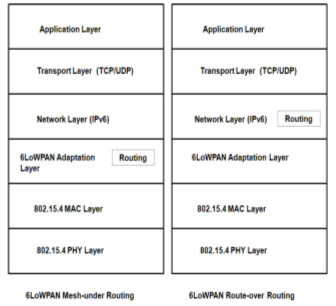
\includegraphics{Route-Over_Mesh-Under.png}
%    \caption{Vergleich zwischen Route-Over und Mesh-Under \cite{route-over_mesh-under}}
%    \label{fig:Route-Over_Mesh-Under}
%\end{figure}

%TODO Vor und Nachteile , warum route over (RPL) besser?
% https://tools.ietf.org/html/draft-routing-architecture-iot-00

% --------------------------------------

\subsection{RPL Ripple: Routing Protocol for Low power and Lossy Networks}
\label{sec: RPL Ripple}

Routing Protocol for Low power and Lossy Networks RPL, auch ``Ripple" genannt, ist ein
Distanzvektor-Routing-Protokoll welches f"ur Verbindungen innerhalb von ``Low power and Lossy Networks" LLNs
konzipiert wurde \cite{rfc6550}. Solche LLNs charakterisieren sich durch Eigenschaften,
wie Beschr"ankungen an Rechnerzeit, Speicher und Stromverbrauch sowie mit Verbindungen mit
geringer Datenrate und allen vorran Instabliti"at und hoher Verlustrate. Diese Eigenschaften
sind dabei fast deckungsgleich mit dennen von LR-WPANs, weshalb RPL f"ur 6LoWPAN angewendet wird.

Die Funktionsweise von RPL zeichnet sich dadurch aus, dass ein zielorientierter, gerichteter,
 azyklischer Graph DODAG (Destination Oriented Directed Acyclic Graph)\cite{rpl_ipso} erstellt wird.
 Dieser DODAG entspricht dabei einer logischen Routing Topologie welches das
 tats"achliche  physikalische Netzwerk abstrahiert. Wobei zu jedem Zeitpunkt
 mehrere DODAGs gleichzeitig auf dem physikalischen Netzwerk liegen k"onnen und jeder
 Graph unterschiedliche Anforderungen und Beschr"ankungen an die Knoten zuweisen kann.
 Dar"uberhinaus kann auf einem Knoten auch mehrere Graphen (RPL Instanzen) gleichzeitig liegen.

Jedem DODAG wird dabei eine Objekt-Funktion zugeordnet, welche dem Graph dadurch
bestimmte Anforderungen und Beschr"ankungen zuweist um den ``besten" Pfad f"ur den
Graphen zu bestimmen. Dieser Prozess wird durch einen Distanzvektoralgorithmus durchgef"uhrt
und arbeitet nach dem Prinzip ``Teile deinen Nachbarn mit, wie du die Welt siehst"\cite{rplwiki}.

Die Knoten eines DODAG operieren dadurch als IPv6 Router, wobei ein Knoten, welcher auf der
Abstraktionsebene von IPv6 an ein anderes Subnetz grenzt, innerhalb des DODAG als Root-Knoten
dient.

Die Anfoderungen entsprechen dabei ausgew"ahlten Metriken, wie ``Ubertragungszeit, Verz"ogerung oder Jitter,
wobei die Beschr"ankungen bestimmte Vorgaben vermeiden, z.B. die Vermeidung Nicht-Verschl"usselter Knoten oder
Batterie-betriebener Knoten.



% neighbour discovery und rpl


% --------------------------------------
% Kapitel 4 - ZigBee und 6LoWPAN
% --------------------------------------

\section{ZigBee und 6LoWPAN}
\label{sec: ZigBee und 6LoWPAN}

Mit ZigBee gibt es bereits seit l"angerem eine propriet"are Spezifikation der
ZigBee Alliance, einem Zusammenschluss von "uber 230 Unternehmen, um den IEEE 802.15.4
Standard auf der Network und Application Layer zu erweitern.

ZigBee war bis zum erscheinen von 6LoWPAN die am verbreiteste Technologie auf dem Markt,
da nicht nur die notwendige softwareseitige Spezifikation erstellt wurde sondern auch
passende Hardware vertrieben wurde.

Im Gegensatz zu 6LoWPAN beschreib ZigBee nicht nur die Anbindung von LR-WPANs mit IPv6,
 sondern baute einen eigenen Network Stack basierend auf IEEE 802.15.4 auf. Die
 Architektur kann in Abbildung \ref{fig:zigbee_protocol_stack} betrachtet werden und beschreibt
 dabei folgende Schichten und Objekte:

\begin{figure}[h]
    \centering
    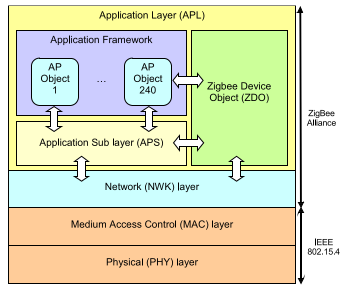
\includegraphics{zigbee_stack.png}
    \caption{ZigBee Protocol Stack basierend auf IEEE 802.15.4 \cite{zigbee_stack_picture}}
    \label{fig:zigbee_protocol_stack}
\end{figure}

\begin{description}
    \item[Network Layer NWK] Die Aufgabe des NWK liegt in der Erstellung, sowie der Organisation
    eiens Mesh Netwerkes basierend auf IEEE 802.15.4 welches abstrahiert wird von dem tats"achlichen
    physikalischen Netzwerk. Das Routing erfolgt dabei "ahnlich zu RPL, indem durch einen Route Discovery Algorithmus,
    dem ``Ad-hoc On Demand Distance Vector Routing Algorithm AODV'' ein Graph erzeugt wird. Dabei "ubernehmen
    Full Function Devices FFD als Knoten im Graphen die Routingaufgaben, indem diese Routing Tabellen RT anlegen und verwalten.

    \item[Application Layer APL] Der APL spezifiziert ein Framework f"ur die Kommunikation und Entwicklung von Anwendungen
    auf dem Application Layer. Der Kernbereich ist dabei das Application Framework, welches bis zu 240 Application Objects APO
    unterst"utzt, benutzerdefinierte Module auf Anwendungsebene. Anhand dieser APOs wurden zwei Sub Layer erschaffen, welche
    verschiedene Aufgaben "ubernehmen. Der ZigBee Device Object ZDO Layer sorgt f"ur die Verwaltung der Kommunikation, des Netzwerkes
    sowie der Netzwerksicherheit, wobei der Application Sub Layer APS den eigentlichen Datentransfer "uberwacht und die Sicherheit
    der Services kontrolliert.

    \item[ZigBee vs. 6LoWPAN] Der direkte Vergleich zwischen beiden Technologien bezieht sich einerseits auf die
    Eigenschaften andererseits auf den wichtigen Punkt der Interoperabilit"at zu anderen Technologien und Protokollen.
    Dabei liegt 6LoWPAN eindeutig im Vorteil, da Interoperablit"at ein wichtiges Designziel war, indem auf IPv6 aufgebaut wurde.
    ZigBee ben"otigt dagegen f"ur die Anbindung an andere Ger"ate bzw. Protokolle eine aufw"andige Schnittstelle auf Anwendungsebene.
    Aber auch die Kerneigenschaften beider Technologien im Vergleich spricht eindeutig f"ur 6LoWPAN, da durch die Routingvariante
    Mesh-Under der Paket Overhead deutlich geringer ist, als beim ZigBee Protokoll. Zus"atzlich ist auch die durchschnittliche
    Implementierung von 6LoWPAN mit 30 KB weitaus gen"ugsamer als die 90 KB von ZigBee.
    Aufgrund dieser Probleme hat die ZigBee Alliance aber durch die Entwicklung  der neuen Spezifikation ZigBeeIP \ref{sec: ZigBeeIP}
    reagiert.
\end{description}

% --------------------------------------

\subsection{ZigBeeIP}
\label{sec: ZigBeeIP}

Mit ZigBeeIP hat die ZigBee Alliance auf das Aufkommen von 6LoWPAN und dem Vorwurf der propriet"aren Software
reagiert. Deshalb wurde eine Spezifikation mit skalierbarer Architektur entwickelt, welche weiterhin auf IEEE
802.15.4 Netzwerken sowie dem IPv6 Networking basiert. Wie die folgende Abbildung \ref{fig:zigbeeip} pr"asentiert
gilt als Grundlage 802.15.4 und darauf aufbauend unabh"angige Standards, wie 6LoWPAN, IPv6 aber auch
 das Routingprotkoll RPL und IPv6 Anwendungen wie Neighbor Discovery sowie Transportprotokolle.
 Durch diese breite Verwendung von Standards wie die Interoperablit"at mit anderen Standards gew"ahrleistet
 und der Fehler eines abgeschlossenen Systems von ZigBee wird nicht wiederholt.
 Aufbauend auf dieser ``super-specification'' \ref{zigbeeip} folgt der ZigBee Smart Energy V2.0 Layer
 ein ip-basiertes Protokoll zur Kontrolle, Monitoring und dem Informationsaustausch von
 Anwendungen. Diese Anwendungen sind teil des urspr"ungliche ZigBee Application Framework
 mitsamt der ZigBee Profiles.

 Durch diese Entwicklung wurde nun eine offene Spezifikation geschaffen, welche vollst"andig auf Standards basiert
 wodurch viele verschiedene Ger"ate innerhalb eines einzigen Kontrollnetzwerkes verbunden werden k"onnen.

\begin{figure}[h]
    \centering
    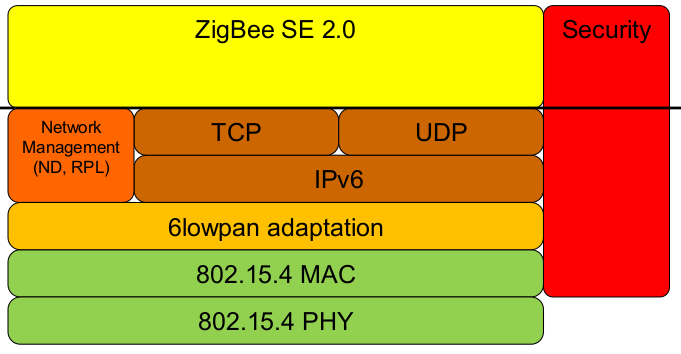
\includegraphics[scale=0.5]{zigbeeip_stack.png}
    \caption{ZigBeeIP Protocol Stack basierend auf IEEE 802.15.4 \cite{zigbeeip}}
    \label{fig:zigbeeip}
\end{figure}

% --------------------------------------
% Kapitel 5 - Zusammenfassung
% --------------------------------------
\section{Fazit}
\label{sec:Fazit}
Abschlie"send kann nun zusammengefasst werden, das durch das Internet der Dinge
und dessen Anforderungen und Beschr"ankungen an die dadurch enstehenden Netzwerke
Protokolle n"otig sind, diese mit vorhandenen Technologien anzubinden.

Deshalb wurde 6LoWPAN entwickelt welches ein Bindeglied zwischen den
IEEE 802.15.4-Netzwerken und IPv6 darstellt. Dabei bildet 6LoWPAN als
Technologie und Kommunikationsprotokoll eine Adapationsschicht um mit dem
``Stacked Header Prinzip'', implementiert durch verschiedene Headertypen, und
einem Kompressionsmechanimus die bis zu 1280 Byte gro"sen IPv6 Pakete an die
127 Byte langen IEEE 802.15.4 Frames anzubinden.

Durch die Kombination beider Technologien, besitzt 6LoWPAN zwei verschiedene
Routingverfahren, den Data Link Layer spezifischen Mesh-Under Routing mittels
MAC-Adressen und dem Standard Routing Verfahren mittels IP-Pakete mitsamt der
Verwendung von Routingprotokollen wie RPL.

Durch diese Eigenschaften wurde damit vom IETF ein fester Standard entwickelt,
um eine Fragmentierung durch mehrere parallel agierende Technologien zu verhindern,
da selbst weit verbreitete, bew"ahrte aber propiet"are Alternativen wie ZigBee
sich an 6LoWPAN anpassen.

% --------------------------------------

% ------------------------------------------------


% ------------------------------------------------
% .... Literaturverzeichnis
% -------------------------
\printbibliography
% ------------------------------------------------
\end{document}
